\chapter{Návrh riešenia}
Na to aby sme boli schopní merať a porovnávať pamäťovú hĺbku sietí, museli sme 
zvoliť vhodné trénovacie dáta, zadefinovať si spôsob merania pamäťovej hĺbky 
sietí a tiež spôsob vyhodnocovania výsledkov.

\section{Metóda uchovávania informácii v SOM}
Na to aby sme boli schopní odmerať pamäťovú hĺbku siete, potrebujeme si pamätať v jednotlivých
neurónoch informáciu o tom, pre ktoré vstupy bol daný neurón víťazom.
Každý neurón bude mať množinu vstupov, v ktorej si pamätá pre aký vstup bol počas trénovania víťazom. 
Nestačí však ukladať iba samotný vstup, pretože by sme prišli o historický kontext pre daný vstup, 
ktorý je nevyhnutný pri určovaní pamäťovej hĺbky.
Preto si neukladáme iba aktuálny vstup (aktuálne písmeno), 
ale $k$ posledných písmen z trénovacej sekvencie.
Toto sa nazýva posuvné okno (ang. sliding window) na vstupnej množine. 
Po natrénovaní siete viem tieto okná vizualizovať ako hitmapu, 
ktorá nám vizualizuje, na ktoré vstupy (resp. okná) neuróny reagovali.

\begin{figure}[H]
	\centering
	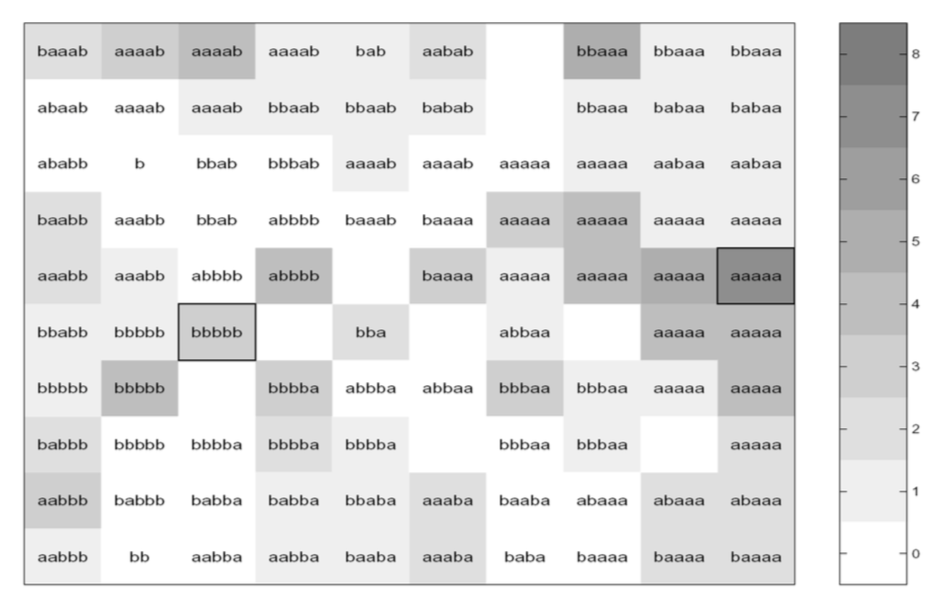
\includegraphics[width=10cm]{assets/receptive_field}
	\caption{Ukážka hitmapy}
\end{figure}
 
\section{Určovanie hĺbky pamäte rekurentnej SOM}
Hĺbku pamäte pre konkrétny neurón v siete určíme ako dĺžku najdlhšej spoločnej
podpostupností písmen v množine posuvných okien vstupov, pre ktoré bol neurón víťazom.
Dĺžku najdlhšej podpostupnosti budeme určovať od konca sekvencií v množine.
Pamäťovú hĺbku celej siete následne určíme ako vážený priemer nameraných pamäťových hĺbok jednotlivých neurónov, 
kde váhami bude počet podpostupností v jednotlivých množinách (teda koľko krát bol nejaký neurón víťazom pre nejaký vstup).
Neuróny, ktoré neboli víťazom pre žiadny vstup sa vo výpočte nezapočítavajú (majú nulovú váhu).
Neuróny, ktoré boli víťazom iba pre jeden vstup, ich pamäťová hĺbka je dĺžka uloženej sekvencie, čiže dĺžka pamäťového okna.
Vo výsledku majú však nízku váhu vzhľadom na iné neuróny.
Priemer pamäťových hĺbok jednotlivých neurónov musí byť vážený, aby neuróny, 
ktoré boli víťazmi pre väčší počet vstupov mali vyššiu váhu ako neuróny, ktoré boli víťazmi pre menší počet vstupov.
Po každej trénovacej epoche (prechode trénovacou množinou) budeme vedieť určiť pamäťovú hĺbku mapy.
Vďaka tomu, že neuróny rekurentných sietí majú okrem normálnych váh aj kontextové váhy, 
ktoré uchovávajú informácie z predchádzajúcich krokov, môže sa stať, že rovnaké písmeno zo vstupu 
bude mať rôzne víťazné neuróny počas trénovania.

Samotná pamäťová hĺbka je relatívna a závisí aj od veľkosti posuvného okna (sliding window).
Veľkosť posuvného okna musí byť dostatočne veľká. Hľadanie dostatočnej veľkosti posuvného
okna je súčasťou nášho experimentu.

\section{Určovanie hĺbky pamäte SRN}
Pri SRN sme skúšali nájsť spôsob ako odmerať pamäťovú hĺbku. 
Navrhli sme riešienie pri ktorom si vizualizujeme vnútorné stavy siete, ale
nevedeli sme rozumne kvantifikovať pamäťovú hĺbku takejto siete. Kontextovú vrstvu v SRN si 
môžeme predstaviť ako veľa viacrozmernú SOM, kde sa zobrazujú informácie zo vstupu
vo viacrozmernom priestore.

Tradeoff medzi rozlišovaciou schopnosťou jednotlivých slov a schopnosťou
zachovať podobné slová topologicky čo najbližšie pri sebe.


% do dalsej kapitoly

\section{Výber vhodných trénovacích dát a ich reprezentácie}
Trénovacie sekvencie sú tvorené písmenami anglickej abecedy (26 písmen).
Spoločnou vlasťnosťou týchto trénovacích množín je, že sú tvorené/generované určitým nenáhodným spôsobom (obsahujú napríklad opakujúce sa podsekvencie)
a teda môžeme na nich trénovať rekurentné neurónové siete. 
Inými slovami dokážu v nich rekurentné neurónové siete zachytiť určité vzory, ktoré si pamätajú vo svojom kontexte.
Samotné vstupy (trénovacie príklady) pre sieť sú zakódované jednotlivé písmená z trénovacej sekvencie.
Keďže neurónové siete vedia najlepšie pracovať iba s číselnými hodnotami, jednotlivé vstupy zo 
vstupnej sekvencie kódujeme počas trénovania do 26 prvkového vektora metódou one-hot, 
a teda jeho prvky sú nuly a jednotka (pre každé písmeno je jednotka na unikátnej pozícii).
Napríklad písmeno A bude reprezentované vektorom
$[1, 0, 0, 0, 0, 0, 0, 0, 0, 0, 0, 0, 0, 0, 0, 0, 0, 0, 0, 0, 0, 0, 0, 0]$,
písmeno B vektorom $[0, 1, 0, 0, 0, 0, 0, 0, 0, 0, 0, 0, 0, 0, 0, 0, 0, 0, 0, 0, 0, 0, 0, 0]$ atď. 
ktorý bude na vstupe neurónovej siete.
Tento spôsob reprezentácie vstupov pre sieť je jednoduchý a siete s ním vedia dobre pracovať.


%
%\section{Hľadanie ideálnych (hyper) parametrov}
%Ako prvé je potrebné zvoliť vhodnú veľkosť posuvného okna na trénovacej množine, tak aby bolo väčšie ako
%najdlhšia nájdená spoločná podpostupnosť znakov. 
%Toto je jednoducho docieliteľné postupným zvyšovaním veľkosti tohto pamäťového okna až pokým pamäťová hĺbka stúpa.

%Ďaľšie dôležité parametre, ktoré potrebujem optimalizovať sú $alpha$ a $beta$ parametre, ktoré
%sa používajú pri počítaní výslednej vzdialenosti vstupného vektora od váhového vektora neurónu.
%Táto vzdialenosť je pri rekurentných SOM určená ako kombinácia vzdialenosti vstupu od váhového vektora neurónu a vzdialenosti
%kontextu od contextového vektora neurónu.
%Jednotlivé parametre určujú akú váhu má aktuálny vstup a akú váhu má kontext pri výpočte výslednej vzdialenosti.
%Toto neviem spraviť nijak inak, iba postupním skúšaním rôznych kombinácii týchto parametrov. 
%$alpha$ aj $beta$.

%Optimálne $alpha$ a $beta$ parameters, ktoré dávajú najlepšie výsledky som hľadal nasledujúcim
%spôsobom:

%Naprogramoval som si skript, pomocou ktorého trénujem sieť s rôznymi parametrami.
%Výsledky som si počas trénovania zaznamenával.
%Následne som si vykreslil 3D grafy pre každý typ trénovanej siete (msom, recsom, vmsom), 
%kde na x-ovej osy sú hodnoty alpha parametra, na y-ovej osy sú hodnoty beta parametra a
%na z-ovej osy sú hodnoty pamäťových hĺbok.
%Na začiatok som zvyšoval parameters po hodnote $0.1$.






